In this chapter, we present a method for the design of an LNA input matching network using automatic differentiation (AD), a technique made popular by machine learning.
The input matching network consists of a non-uniform suspended stripline transformer, directly optimized with AD-provided gradients.
Compared to the standard approach of finite-differences, AD provides orders of magnitude faster optimization time for gradient-based solvers.
This dramatic speedup reduces the iteration time during design and enables the exploration of more complex geometries.
The LNA designed with this approach improves over a previous two-section uniform-line design, achieving an average noise temperature of \newnoise over the frequency range of \qtyrange{0.7}{2}{\GHz} at room temperature.
We optimized the geometry in under \qty{5}{\s}, \num{40}x faster than optimizing with finite-differences.

\section{Introduction}

Radio telescope receivers are typically cooled to give high sensitivity, but the cost of cooling is prohibitive for arrays of thousands of telescopes.
Receivers with ambient-temperature LNAs are becoming competitive with cooled designs at low frequencies, resulting in dramatically decreased cost that enables the development of enormous arrays such as the DSA-2000~\cite{hallinanDSA2000RadioSurvey2019}.
A key metric for these arrays is the speed at which they create images of the sky.
The observation time required for some fixed noise in an image is $\propto T^2$, where $T$ is the system noise temperature.
At decimeter wavelengths, LNA noise typically dominates the system noise~\cite{flygareWidebandLowLossFeed2024}, so even \qty{1}{\K} improvement in the LNA significantly increases the survey speed and subsequent science return.
The key LNA development has been the use of a low-noise transistor from Diramics~\cite{DiramicsPH2004F50} with a low-loss suspended stripline input matching network~\cite{weinrebLowNoiseAmplifier2021, shiRoomTemperatureLowNoiseAmplifier2023}, consisting of uniform transmission line (UTL) transformers.
We have improved the LNA noise temperature by changing the input matching network to a non-uniform transmission line (NTL).

It is well known that NTLs are useful in wideband matching and are easily implemented in suspended stripline.
For our LNA, an NTL gives a better trade-off between insertion loss and noise match, but designing such a line is nontrivial.
The geometry must be directly optimized in situ, as no closed-form expression for the desired behavior of the NTL exists.

To optimize the geometry of the NTL, we follow the standard practice of gradient descent.
In most electronic design automation (EDA) packages, the gradient is approximated via finite-differencing, but finite-differencing is imprecise and inefficient for large-dimensional optimization, as is the case for an NTL problem.
While direct optimization is a common technique in designing NTLs~\cite{miazgaNonuniformTransmissionLine2014, miazgaDiscreteShapeOptimization2008, schaepperleOptimizationDistributedParameter1994}, the performance overhead of computing the gradient is a limiting factor.

Instead of computing the gradient with finite-differencing, we used automatic differentiation (AD)~\cite{baydinAutomaticDifferentiationMachine2017}, an algorithmic tool made popular by machine learning.
AD is an accelerated way to compute the exact derivatives of an arbitrary computer program.
As AD is an exact method, it is more precise than finite-differencing and typically higher performance.
Gradient-descent optimization of NTLs with AD dramatically reduces optimization time, which enables more complex designs.

In this chapter, we describe the design, implementation, and experimental verification of an LNA whose input matching network is an NTL designed via direct optimization using AD.
The NTL design achieves lower average noise temperature than the UTL design.
Optimization of the NTL took under \qty{5}{\s}, \num{40}x faster than solving the equivalent finite-differenced gradient-based problem in a commercial EDA package.

In \autoref{sec:math}, we discuss this mathematical formulation in detail with an overview of the LNA design problem posed as constrained nonlinear optimization, the AD method, and NTL design.
In \autoref{sec:impl}, we discuss the implementation details of applying this technique to our LNA design.
Finally, in \autoref{sec:measurement}, we present experimental results to demonstrate the performance of the amplifier.

\section{Mathematical Formulation} \label{sec:math}

\subsection{Low-Noise Amplifier Optimization}

The priority for any LNA design is to minimize the amplifier's noise.
Balancing this priority with other requirements such as input reflection, stability, gain, etc. is application-specific and is stated mathematically as
%
\begin{mini}
	{\GS}{F(\FMin, R_n, \GOpt, \GS)}
	{}{}
	\addConstraint{G(\mathbf{S}, \GL, \GS)}{\leq \xi}
	\label{eqn:optim}
\end{mini}
%
where $F$ is the noise objective function, given here in the standard form of noise figure~\cite{gonzalezMicrowaveTransistorAmplifiers1997}, driven by the device's noise parameters via
%
\begin{equation}
	F = \FMin + \frac{4R_{n}\left|\GS-\GOpt\right|^{2}}{Z_{0}\left|1+\GOpt\right|^{2}\left(1-\left|\GS\right|^{2}\right)}
	\label{eq:noise}
\end{equation}
%
where $\FMin$ is the minimum noise figure, $R_{n}$ is the noise equivalent resistance, and $\GOpt$ is the optimum source reflection coefficient that results in $\FMin$.
$G$ is the constraint, a function of the transistor's S parameters, $\mathbf{S}$, and input and output reflection coefficients, $\GS$ and $\GL$, shown in \autoref{fig:fet_gammas}.
The constraint function captures any of the non-noise requirements and is represented by an inequality with some scalar $\xi$.
The solution to \eqref{eqn:optim} is the $\GS$ that minimizes the noise figure given a biased transistor's S and noise parameters under some constraint.
Notably, the solution gives minimum noise without specifying any goal or target.
It is then up to the designer to evaluate the result and determine if it is satisfactory, loosening the constraints as necessary.
This is distinct from ``goal-based'' optimization, where the optimizer attempts to solve a potentially unfeasible problem and returns a goal-weighted least-squares solution.

If we were only interested in constraining input reflection, we would define $\xi$ as a maximum allowed magnitude of $\GA$ and write our constraint function as
%
\begin{equation}
	G \leq\left|\GA\right|_{\text{Max}}
	\label{eq:ga_constraint}
\end{equation}
Alternatively, we could constrain the gain to be greater than some value, either case being a trade-off between power and noise match.
In this work, we will constrain $|\GA|$.
%
\begin{figure}[t]
	\centering
	\begin{circuitikz}[european]
		\tikzstyle{every node}=[font=\LARGE]
		\draw (4.5,12.25) to[Tnmos] (4.5,14.25);
		\draw (3.65,13.25) to[short] (3.5,13.25);
		\draw  (1.5,14.5) rectangle (3,12);
		\draw  (5.25,14.5) rectangle (6.75,12);
		\draw [short] (4.5,14.25) -- (5.25,14.25);
		\draw [short] (3,12.25) -- (5.25,12.25);
		\draw (7.25,14) to[R] (7.25,12.5);
		\node [font=\small] at (7.25,13.25) {$Z_{L}$};
		\draw (3.5,13.25) to[short] (3.5,14.25);
		\draw (3.5,14.25) to[short] (3,14.25);
		\draw (1,14) to[R] (1,12.5);
		\node [font=\small] at (1,13.25) {$Z_{S}$};
        
		\node [font=\large] at (2.25,13.25) {IMN};
		\node [font=\large] at (6,13.25) {OMN};
        
		\draw [->, >=Stealth] (3.25,12.5) -- (3.5,12.5);
		\draw [short] (3.25,12.5) -- (3.25,12);
		\node [font=\small] at (3.25,11.75) {$\Gamma_{\text{In}}$};
        
		\draw [short] (5,12.5) -- (5,12);
		\draw [->, >=Stealth] (5,12.5) -- (4.75,12.5);
		\node [font=\small] at (5,11.75) {$\Gamma_{\text{Out}}$};
		\node [font=\small] at (1.25,11.75) {$\Gamma_{\text{A}}$};
		\node [font=\small] at (1.25,12.5) {};
		\draw [->, >=Stealth] (1.25,12.5) -- (1.5,12.5);
        
		\draw (1.25,12.5) to[short] (1.25,12);
		\draw [->, >=Stealth] (7,12.5) -- (6.75,12.5);
		\node [font=\small] at (7,11.75) {$\Gamma_{\text{B}}$};

        \draw [->, >=Stealth] (1.25,14) -- (1,14);
		\draw (1.25,14) to[short] (1.25,14.5);
		\node [font=\small] at (1.25,14.75) {$\Gamma_{\text{S}}$};
        
		\draw [->, >=Stealth] (3.25,14) -- (3,14);
		\draw (3.25,14) to[short] (3.25,14.5);
		\node [font=\small] at (3.25,14.75) {$\Gamma_{\text{S}}^\prime$};
        
		\draw [->, >=Stealth] (5,14) -- (5.25,14);
		\draw [short] (5,14) -- (5,14.5);
		\node [font=\small] at (5,14.75) {$\Gamma_{\text{L}}^\prime$};

        \draw [->, >=Stealth] (7,14) -- (7.25,14);
		\draw [short] (7,14) -- (7,14.5);
		\node [font=\small] at (7,14.75) {$\Gamma_{\text{L}}$};

        
		\draw [short] (7,12.5) -- (7,12);
		\draw (1,14) to[short] (1,14.25);
		\draw (1,14.25) to[short] (1.5,14.25);
		\draw (1,12.5) to[short] (1,12.25);
		\draw (1,12.25) to[short] (1.5,12.25);
		\draw (7.25,14) to[short] (7.25,14.25);
		\draw (6.75,14.25) to[short] (7.25,14.25);ragged
		\draw (6.75,12.25) to[short] (7.25,12.25);
		\draw (7.25,12.5) to[short] (7.25,12.25);
	\end{circuitikz}
	\caption{Reflection planes for a typical microwave transistor amplifier, its input matching network (IMN) and output matching network (OMN)}
	\label{fig:fet_gammas}
\end{figure}

The optimal $\GS$ solution, however, is only valid at a single frequency and could be readily solved by hand.
In practice, we sample the device's S and noise parameters across a set of $N$ discrete frequency points, $\nuvec$, and our goal is to design an amplifier that operates over a subset of that range.
For this wideband LNA design, one formulation is to minimize the average noise
%
\begin{mini}
	{\GS(\nuvec)}{\frac{1}{N}\sum_{i=1}^{N} F(\nu_i)}
	{}{}
	\addConstraint{G(\nuvec)}{\leq\left|\GA\right|_{\text{Max}}}
	\label{eqn:optim_geo}
\end{mini}
%
Here, the minimizer and constraints are vector-valued.
In this form, \eqref{eqn:optim_geo} is a constrained, weighted, nonlinear least-squares problem, as minimizing the average noise figure over $\GS(\nuvec)$ is proportional to minimizing the $R_n$-weighted mean squared distance between $\GS(\nuvec)$ and $\GOpt(\nuvec)$, subject to the input reflection constraint.

In practice, the $\GS(\nuvec)$ solution is not directly useful, as ultimately, we aim to design the network that induces $\GS(\nuvec)$.
Therefore, instead of minimizing over $\GS(\nuvec)$, we minimize over the input matching network directly.
If, for example, this matching network were a series UTL with electrical length $l$, phase constant $\beta$, and characteristic impedance $Z_L$, the problem becomes
\begin{mini}
	{l, Z_L}{\frac{1}{N}\sum_{i=1}^{N} F({\GS}(\nu_i))}
	{}{}
	\addConstraint{G({\GS}(\nuvec))}{\leq\left|\GA\right|_{\text{Max}}}
	\label{eqn:optim_line}
\end{mini}
%
where
\begin{equation}
	\GS(\nu) = Z_0\left[\frac{Z_L +jZ_0\tan\left(\beta(\nu)l\right)}{Z_0 +jZ_L\tan\left(\beta(\nu)l\right)}\right]
\end{equation}
%
Here, we reduce the dimensionality of the problem from $N$ to two as we are solving for a single length and characteristic impedance.
However, there is no guarantee that this topology achieves the same average noise figure as the optimum $\GS(\nuvec)$ solution.
Solving this transformed problem is now akin to regression, as the structure of the matching network dictates the frequency response and the solver will try to ``curve fit'' that frequency response to the optimum $\GS(\nuvec)$ solution.
Selecting an appropriate network topology is therefore crucial for achieving optimal results.
In this work, we investigate NTLs as a general-purpose topology.

With a chosen a topology, we solve the minimization problem with gradient-based nonlinear optimization.
The inclusion of an inequality in the constraint \eqref{eq:ga_constraint} implies the solver must contend with a system of Karush-Kuhn-Tucker (KKT) conditions~\cite{kuhnNonlinearProgramming1951} and therefore must be solved numerically.
Gradient-based KKT solvers will evaluate the cost function, the constraints, and the gradient/Jacobian potentially thousands of times.
Computing these values efficiently is essential to the performance of this design method.

\subsection{Automatic Differentiation}

Traditionally, there are three ways one can generate gradients for optimization.
First, if the cost expression is simple, one could solve the gradient by hand by applying the rules of calculus.
However, if the expression were large or if it were a black-box with unknown internals, deriving an expression for the gradients might be impossible.
The second approach is to approximate the gradient via finite-differencing each term using the standard form:
%
\begin{equation}
	\frac{df}{dx} \approx \frac{f(x+h)-f(x)}{h}
	\label{eqn:finite-difference}
\end{equation}
%
This is a simple formulation which works on any well-behaved function and is the solution of choice for most EDA software.
However, these approximations suffer from numeric instability and high sensitivity to the choice of the step size $h$~\cite{jerrellAutomaticDifferentiationInterval1997}.

The third option is to use a computer algebra system to perform ``symbolic differentiation''.
This method applies the rules of calculus to an expression tree and is a simple mechanistic process for computers.
However, the complexity of computing a symbolic result grows exponentially with the number of terms, resulting in a problem known as ``expression swell''~\cite{corlissApplicationsDifferentiationArithmetic11988}.
For optimization, we are not interested in the symbolic form as we only need an accurate numeric gradient to know the direction of steepest descent, so this extra computation is not useful.

Automatic differentiation (AD) is a technique distinct from the aforementioned approaches, where a program algorithmically computes derivatives via the accumulation of values during execution.
This method is not an approximation like \eqref{eqn:finite-difference}, nor does it generate expressions like symbolic differentiation.
While there are several implementation strategies, the general formulation yields accurate gradients to machine precision with a small, constant overhead.
As AD operates on values rather than expressions, it can be applied to most programs, including those that utilize loops, branching statements, and recursion.
Efficient implementations of AD have been transformational in the machine learning community, where large, complex models composed of arbitrary code can be differentiated and optimized~\cite{pytorch}.
From the AD perspective, a program that computes circuit behavior (noise, gain, etc.) is no different from a program that implements a machine learning model, as both are composed of simple, differentiable pieces.

% Do we keep this in here?
The application of AD to circuits is not a new idea, but is surprisingly underutilized.
As noted in~\cite{feldmannAutomaticDifferentiationCircuit1992}, ``[AD] can enable applications previously deemed impractical''.
While AD has not had much exposure outside of machine learning, it has been recently used for parameter estimation of lumped-element circuit models~\cite{mezzaDataDrivenParameterEstimation2023a} and sensitivity analysis of EM structures~\cite{toivanenElectromagneticSensitivityAnalysis2009}.
Some older works conclude the performance overhead may not justify use over finite-differences, but the explosion in machine learning research has accelerated the development of high-performance AD libraries.

AD operates by decomposing a complex function into a sequence of simple operations with known derivatives.
As the function is evaluated, AD propagates these derivatives via the chain rule.
The chain rule states that each subsequent derivative is multiplied by the previous.
As multiplication is associative, we can compute the total derivative from input to output or vice versa.
This leads to the two modes of AD: forward-mode and reverse-mode.

In forward-mode, derivatives are computed as the function is evaluated, starting with the input independent variables.
Each operation in the function is evaluated along with its derivative with respect to the input, which propagates forward to compute the final derivative.
This method is efficient when the function has few inputs and many outputs, as each input's derivative must be propagated through the function one at a time, similar to finite-differences.
In reverse-mode, the function is first evaluated normally, and then derivatives are propagated backward from the outputs to inputs, using the chain rule to accumulate derivatives with respect to each input.
This is identical to the familiar ``backpropagation'' algorithm used in training neural networks.
Reverse-mode is particularly efficient for functions with few outputs and many inputs, such as machine learning, where the goal is often to compute gradients of a scalar loss function with many parameters.
The same is true for this work, where circuit optimization manifests as high dimensional optimization of a scalar cost function.
In either mode, AD computes exact derivatives and is more computationally efficient compared to traditional numerical differentiation methods.
A more complete mathematical treatment of AD is given in \autoref{ch:ad_appen}.

\subsection{Non-Uniform Transmission Lines}

Non-uniform transmission lines (NTLs) are a class of transformer structures used in many microwave circuits.
These transmission lines vary their impedance continuously as a function of position to achieve such goals as matching~\cite{xiaoImpedanceMatchingComplex2002}, filtering~\cite{panArbitraryFilterDesign1999}, or miniaturization~\cite{khalaj-amirhosseiniNonuniformTransmissionLines2008}.
% Reviewer 1.3 - Explain how NTLs were not chosen just because it works well with AD
For ambient-temperature LNAs designed around very low noise transistors, minimizing the loss of the input matching network is essential.
As discussed in~\cite{weinrebLowNoiseAmplifier2021}, suspended stripline matching structures provide the lowest loss.
Implementing the suspended stripline as an NTL is a natural development of the stepped transformer in~\cite{shiRoomTemperatureLowNoiseAmplifier2023} and empirically results in a lower noise temperature.
Other strategies such as lumped matching are simply too lossy and are not considered for this work.

Unfortunately, the scattering behavior for a general NTL has no analytic form.
This arises from the fact that for a general transmission line, the voltage and current as a function of position are governed by a set of Riccati differential equations~\cite{sugaiRiccatiBernoulliEquations1961}.
While closed-form solutions exist for special cases, such as exponential tapers~\cite{wheelerTransmissionLinesExponential1939}, a standard approach for analyzing arbitrary NTLs is to discretize the line into many small lengths of constant impedance sections.

We represent the discretized approximation of an NTL as the multiplication of ABCD (cascade) matrices of the uniform sections~\cite{maoAnalysisTimeResponse1992}.
For a uniform transmission line of length $l$ with characteristic impedance $Z_c$ and propagation constant $\gamma$, this matrix is:
%
\begin{equation}
	\mathbf{A}\left(Z_c,\gamma,l\right) = \begin{bmatrix}
		\cosh{\gamma l}                & Z_{c}\sinh{\gamma l} \\
		1/Z_c\sinh{\gamma l} & \cosh{\gamma l}
	\end{bmatrix} = \begin{bmatrix}
		A & B \\
		C & D
	\end{bmatrix}
	\label{eqn:tl_abcd}
\end{equation}
%
For an NTL defined by a characteristic impedance and propagation constant profile with position, $Z_c(x), \gamma(x)$, and total length $L$, we pick a discretization of $M$ points and compute:
%
\begin{equation}
	\mathbf{A}_{\text{NTL}} \approx \prod_{i=1}^{M} \mathbf{A}\left(Z_c\left( iL/M \right),\gamma\left(iL/M \right),L/M \right)
	\label{eqn:ntl_casc}
\end{equation}
%
We convert this final ABCD matrix into scattering parameters via
\begin{equation}
	\mathbf{S} = \frac{1}{\zeta}
    \begingroup % keep the change local
    \setlength\arraycolsep{2pt}
	\begin{bmatrix}
		A + B/Z_0 - CZ_0 + D & 2(AD-BC)          \\
		2                            & -A + B/Z_0 - CZ_0 + D
	\end{bmatrix}
    \endgroup
	\label{eqn:a2s}
\end{equation}
where
\begin{equation}
	\zeta = A + B/Z_0 + CZ_0 + D
\end{equation}
and $Z_0$ is the reference impedance for the S parameters and reflection coefficients in the design.

To design an NTL for some particular function, we can optimize the set of discrete impedances that approximate the NTL~\cite{miazgaNonuniformTransmissionLine2014}.
In this case, we are solving the “inverse problem” of finding the discretized $Z_c(x)$ that yields some behavior.
To perform this optimization, we take the set of impedances, compute the two-port scattering behavior via \eqref{eqn:ntl_casc} and \eqref{eqn:a2s}, and use this result to compute an error function against the desired behavior.
For gradient-based optimization, we need the gradient of this error function with respect to the set of impedances.

For an $M$-section discretization of an NTL, a program needs to evaluate $M-1$ matrix multiplications.
Then, for the finite-difference method (or forward-mode AD), the program evaluates the sensitivity of the cost function with respect to every $M$ section.
These combined operations, performed for every iteration of an optimizer, have an algorithmic complexity of $\mathcal{O}(M^2)$.
This scaling dramatically increases the optimization time of designs with large $M$.
However, large $M$ is desirable as it reduces error due to discretization.
With reverse-mode AD, which “back-propagates” the sensitivity of the cost function to the inputs, the complexity of computing the gradient is constant over $M$.
This results in an optimization complexity of $\mathcal{O}(M)$.

\begin{figure}[t]
	\centering
	\begin{tikzpicture}
		\begin{axis}[xlabel={Number of Sections (M)},
				ylabel={Runtime (s)},
				width=13cm,
				height=6cm,
				xmode=log,
				ymode=log,
                grid=both,
                xmin=1e0,xmax=1e5,
                ytick={1e-7, 1e-5, 1e-3, 1e-1, 1e1, 1e3},
                grid style={line width=.1pt, draw=gray!10},
                major grid style={line width=.2pt,draw=gray!50},
				legend pos={north west},]
			\addplot[mark=none] table [x=n, y expr=1e-9*\thisrow{time}, col sep=comma] {reverse_bench.csv};
			\addplot[mark=none, red, dashed, very thick] table [x=n, y expr=1e-9*\thisrow{time}, col sep=comma] {forward_bench.csv};
			\addplot[mark=none, blue, dotted, very thick] table [x=n, y expr=1e-9*\thisrow{time}, col sep=comma] {finite_bench.csv};
			\legend{Reverse-Mode AD, Forward-Mode AD, Finite-Difference}
		\end{axis}
	\end{tikzpicture}
	\caption{Experimental verification of runtime speed of gradient computation for various methods versus NTL discretization}
	\label{fig:grad_speed}
\end{figure}

The massive speedup of computing the gradients using reverse-mode AD results in orders of magnitude faster NTL optimization.
To demonstrate this, we computed the gradient of a simple scalar cost function ($|S_{11}|^2$) with respect to an $M$-discretized NTL of constant length.
The runtime of this computation versus $M$ is shown in \autoref{fig:grad_speed}.
For a typical $M$ of \num{100} sections~\cite{raeAnalysisStraightTapered1977}, reverse-mode AD yields gradients two orders of magnitude faster than forward-mode and without the numerical error of finite-differencing.
% In a reproduction of optimizing a real-to-real impedance transformer following~\cite{miazgaNonuniformTransmissionLine2014} with a fixed number of iterations, we achieve equivalent results in \qty{100}{\ms} with reverse-mode AD versus \qty{10}{\s} for finite-differences.

The utility of this direct-optimization method extends beyond solving the $Z_c(x)$ profile.
To implement the NTL, one would use the $Z_c(x)$ result to synthesize physical dimensions.
This problem is ill-posed, as realistic transmission lines have coupled $Z_c$ and $\gamma$, both of which are functions of frequency.
A simpler approach is instead to optimize the geometry directly~\cite{miazgaDiscreteShapeOptimization2008, schaepperleOptimizationDistributedParameter1994}.
The geometry induces a $Z_c$ and $\gamma$, which is then used in \eqref{eqn:ntl_casc}.

Recent work~\cite{tremuelParameterfreeNeuralFieldbased2023} has shown another strategy, using convolutional neural networks to capture the geometry-driven behavior of an NTL which is then used for optimization-based inverse design.
However, this method is resource-intensive as it relies on many full-wave simulations of ``example'' lines as well as network training.
While the simple cascade method that we use suffers from the $M$-discretization, it does not require training, or lengthy EM simulations, and is therefore much faster.

To perform the direct geometry optimization, we start with the per-unit-length equivalent resistance, inductance, conductance, and capacitance (RLGC) model of a transmission line with
%
\begin{equation}
	\gamma = \sqrt{\left(R + j \omega L\right) \left( G + j \omega C\right)}
\end{equation}
%
\begin{equation}
	Z_{c} = \sqrt{\left(R + j \omega L\right) / \left( G + j \omega C\right)}
\end{equation}
%
This model captures all the effects of loss and dispersion.
While some transmission lines like coax have an analytic RLGC form, in general, we use curve-fit models.
These models can be frequency-dependent, and are readily extracted from measured data or EM simulations~\cite{zhangCausalRLGCModels2010}.
For suspended stripline, we parameterize this model by widths of the center conductor $\mathbf{W}$ and total length $L$, as the mechanical design dictates fixed height, dielectric constant, etc.
The model also enables constraints on geometry like maximum/minimum length or width.
These constraints should be kept loose to maximize the likelihood of finding an optimal design.

We apply the NTL direct optimization method to our LNA problem via
\begin{mini}
	{L, \mathbf{W}}{\frac{1}{N}\sum_{i=1}^{N} F({\GS}(\nu_i, \mathbf{W}, L))}
	{}{}
	\addConstraint{G({\GS}(\nuvec, \mathbf{W}, L))}{\leq\left|\GA\right|_{\text{Max}}}
	\label{eqn:optim_ntl}
\end{mini}
%
where $\GS$ follows \eqref{eqn:a2s}.
Here, the geometry of the NTL is the domain over which we solve the nonlinear least squares problem from before.
This benefits our LNA design in that we simultaneously account for both the match to $\GOpt$ and the insertion loss of the line itself.
This proves to be critical to the design, as the insertion loss of the input matching network is close in magnitude to the minimum noise figure of the transistor.
The direct optimization approach balances the two sources of noise to result in an optimal design.

\section{Implementation} \label{sec:impl}
% Comment 1.3 - Explain why the changes in structure warrant a fair comparison
To design the improved amplifier, we started with the design from~\cite{shiRoomTemperatureLowNoiseAmplifier2023}.
We make use of the same \qty{400}{\nm} x \qty{200}{\um} gate, four-finger transistor from Diramics~\cite{DiramicsPH2004F50} at a slightly lower bias of $V_d$=\qty{0.5}{\V}, $I_d$=\qty{16}{\mA} to match the vendor's updated model.
To improve linearity, we changed to a two-stage design versus the three-stage design of the prior work.
We also replaced the second stage with a higher current transistor with near identical noise, the SAV-541+ from Mini-Circuits.
As the first stage provides more than \qty{20}{\dB} of gain, the noise of the amplifier is practically independent of these modifications.
These changes result in an amplifier with better linearity and slightly lower gain.
Lastly, we borrow the general chassis geometry for the suspended stripline input matching network.
Apart from these similarities, the designs are independent.
The goal for this design was to improve the noise while maintaining similar gain and $S_{11}$ over the same bandwidth of \qtyrange{0.7}{2}{\GHz}.

For the suspended stripline input, we chose the dimensions to satisfy a few conditions.
First, the total height of the completed amplifier must be \qty{<= 20}{\mm} to satisfy a mechanical constraint for the telescope feed design.
Second, the substrate must be close to the centerline of the amplifier to accommodate connectors.
Finally, the distance between the substrate and the top and bottom ground planes should be close to equal to minimize the average current density and therefore insertion loss.
The large substrate to ground spacing allows for the construction of very high impedance sections, as is required for this particular design due to the transistor's high $Z_{\text{Opt}}$.
The resulting model cross-section geometry is shown in \autoref{fig:cross_section}.
The substrate material is \qty{0.508}{\mm}-thick RT/duroid 5880 with \qty{0.5}{\ounce} cladding.
We chose a surface finish of electroless palladium / immersion gold (EPIG) over rolled copper to minimize surface roughness, to eliminate lossy nickel, and to provide a suitable surface for wire bonding.

\begin{figure}
	\centering
	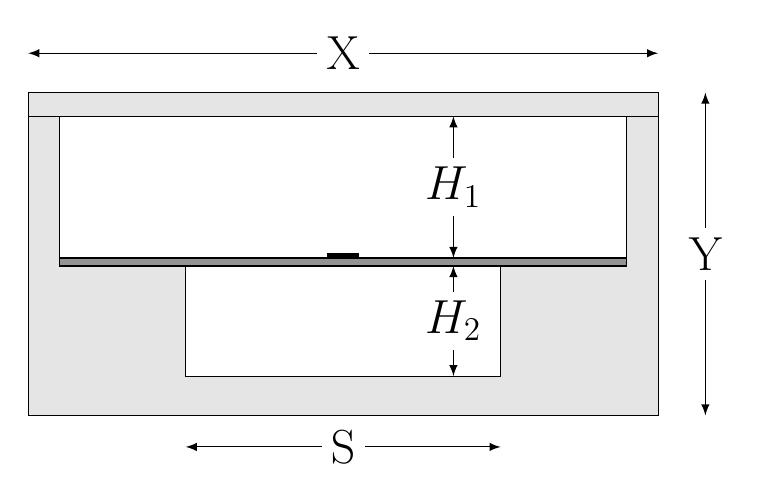
\begin{tikzpicture}[scale=0.2]
		% Case
		\draw[fill=gray!20] plot coordinates
			{(0,0) (0,-19) (40,-19) (40,0) (38,0) (38,-9.508) (30,-9.508) (30,-16.508) (10,-16.508) (10,-9.508) (2,-9.508) (2,0) (0,0)};
		% PCB
		\draw[fill=gray!85] plot coordinates  {(2,-9.508) (2,-9) (38,-9) (38,-9.508) (2,-9.508)};
		% Trace
		\draw[fill=black] plot coordinates {(19,-9) (21,-9) (21,-8.7) (19, -8.7) (19,-9)};
		% Lid
		\draw[fill=gray!20] plot coordinates {(0,0) (0,1.5) (40,1.5) (40,0) (0,0)};
		% Body Dimensions
		\draw[latex-latex] (0,4) -- (40, 4) node[midway,fill=white]{X};
		\draw[latex-latex] (43,1.5) -- (43, -19) node[midway,fill=white]{Y};
		% SS Dimensions
		\draw[latex-latex] (27,-9.508) -- (27, -16.508) node[midway,fill=white]{$\text{H}_2$};
		\draw[latex-latex] (27,0) -- (27, -9) node[midway,fill=white]{$\text{H}_1$};
		\draw[latex-latex] (10,-21) -- (30, -21) node[midway,fill=white]{S};
	\end{tikzpicture}
	\caption[Cross-section of the suspended stripline with critical dimensions]{Cross-section of the suspended stripline with critical dimensions. X=\num{33}, Y=\num{20}, S=\num{20}, $\text{H}_1$=\num{9.5}, $\text{H}_2$=\num{7}, all values in \si{\mm}.}
	\label{fig:cross_section}
\end{figure}

We drew the stripline geometry in ANSYS's 2D Extractor, and solved for the RLGC parameters as a function of frequency from \qtyrange{0.1}{3}{\GHz} in \num{51} uniform steps and as a function of trace width from \qtyrange{0.05}{15}{\mm} swept logarithmically with \num{111} steps per decade.

Next, we designed the section of the amplifier following the input matching network in Keysight's Advanced Design System (ADS).
We used models of lumped components from Modelithics and the Diramics-provided model of the first stage transistor.
This section of the design was unremarkable and used standard techniques.
We used resistive matching to achieve wideband, high output return loss.
We accomplished interstage matching with a single series capacitor.
We designed the second stage active bias following the vendor's recommendation.
Once we completed this design, we created a layout to perform a full wave EM co-simulation with the component circuit models, a crucial step in solving layout-related stability issues.
Finally, we exported the partial amplifier S and noise parameters for the final optimization step of this work.
The schematic for the amplifier is shown in \autoref{fig:schematic}.

\begin{figure}[t]
	\centering
	\begin{tikzpicture}
		\ctikzset{nodes width/.initial=0.1}
		\ctikzset{bipoles/length=0.8cm}
		\ctikzset{nodes width/.initial=.05}

		\draw (0,0) node[bnc](In){} to[C=C1, -*] ++(1,0) coordinate (Gin)
		(Gin) to[L=L1] ++(0,2.2) to[short,-o] ++(0,0) node[above]{$v_{g1}$}
		(Gin) to[mstline, mstlinelen=0.9, l=IMN] ++(1,0) coordinate (Q1G)
		(Q1G) -- ++(0,0) node[nigfetd, anchor=G](Q1){}
		(Q1.S) -- ++(0,0) node[ground]{}
		(Q1.D) -- ++(0.0,0) node[short]{} coordinate (Q1D)
		(Q1D) to[L=L2, *-] ++(0,1.6) to[short,-o] ++(0,0) node[above]{$v_{d1}$}
		(Q1D) to[C, l_=C2] ++(1,0) coordinate (Vg2)
		(Vg2) to[R=R1, *-] ++(0,1.6) to[short,-o] ++(0,0) node[above]{$v_{g2}$}
		(Vg2) -- ++(0.2,0) node[nigfetd, anchor=G](Q2){}
		(Q2.S) -- ++(0,0) node[ground]{}
		(Q2.D) -- ++(0.0,0) node[short]{} coordinate (Q2D)
		(Q2D) to[L,l_=L3, *-] ++(0,1) to[short,-o] ++(0,0) node[above]{$i_{d2}$}
		(Q2D) to[C,l_=C3] ++(1,0) to[L=L4] ++(0.9,0) coordinate (out_match)
		(out_match) to[R,l_=R2,*-] ++(0,-1) to[L, l_=L5] ++(0,-0.7) to ++(0,0) node[ground]{}
		(out_match) to[C=C4] ++(1,0) node[bnc, rotate=-180](Out){} ;
	\end{tikzpicture}
	\caption[Schematic of the RF-portion of the LNA]{Schematic of the RF-portion of the amplifier. C1=3x\qty{47}{\pF}, C2=\qty{2.5}{\pF}, C3=\qty{2}{\pF}, C4=\qty{20}{\pF}, L1=\qty{100}{\nH}, L2,L3=\qty{120}{\nH}, L4=\qty{2}{\nH}, L5=\qty{4.7}{\nH}, R1=5.1k$\Omega$, R2=41.2$\Omega$} %fixme hack for JMW
	\label{fig:schematic}
\end{figure}

\begin{figure}[t]
	\centering
	\begin{tikzpicture}
		\begin{axis}[ymin=-10,
        ymax=10,
        unit vector ratio*=1 1,
        width=13cm,
        xlabel=X (\si{\mm})
        ylabel=Y (\si{\mm})]
			\addplot [name path=upper,draw=none] table[x expr=\thisrow{x}*1000,y expr=\thisrow{y}/2*1000, col sep=comma] {shape.csv};
			\addplot [name path=lower,draw=none] table[x expr=\thisrow{x}*1000,y expr=-\thisrow{y}/2*1000, col sep=comma] {shape.csv};
			\addplot [fill=black] fill between[of=upper and lower];
		\end{axis}
	\end{tikzpicture}
	\caption{Optimized NTL input matching network}
	\label{fig:shape}
\end{figure}

We wrote the NTL optimization code in the Julia programming language~\cite{bezansonJuliaFreshApproach2017a}, an open-source, high-level, high-performance language for scientific computing.
This language has an extensive ecosystem in both AD and in nonlinear optimization.
Further, the AD implementations in Julia typically outperform implementations in other languages.

In Julia, we collected the RLGC data from the 2D EM simulation, as well as the S and noise parameters from the circuit simulation.
We used the RLGC data to create a linear interpolation across width and frequency for each parameter.
We constructed the optimization problem with \textit{Optimization.jl}.
This package exposes a structure for defining arbitrary, constrained optimization problems that provide their gradients using a pluggable AD backend.
We used the state-of-the-art package \textit{Enzyme.jl}~\cite{mosesInsteadRewritingForeign2020} as the reverse-mode AD backend as-is with no modifications.
We limited the optimization domain to widths between \qty{0.1}{\mm} and \qty{15}{\mm} and lengths between \qty{50}{\mm} and \qty{120}{\mm}.
We set the constraints such that the input return loss was greater than \qty{\sim9}{\dB} for every point in frequency, representing a compromise between match and noise.

We solved the optimization problem for \num{100} sections, with an initial profile of a \qty{100}{\mm}-length linear taper from \qty{15}{\mm} to \qty{0.1}{\mm} using the \textit{Ipopt} solver~\cite{wachterImplementationInteriorpointFilter2006}.
On an Intel Xeon Gold 6128 workstation, \num{50} iterations were completed in under \qty{5}{\s}.
As gradient-based optimization only finds a local minimum, we ran the optimizer from different starting vectors to compare a few different results.
The problem was robust against initial conditions, as solving with different starting profiles resulted in similar line shapes of equal performance.
% This aligns with the conclusion from~\cite{miazgaDiscreteShapeOptimization2008}, where discrete shape optimization ``seems to be convex''.
In the worst initial case of random widths, the solver took around 2x longer to converge.
However, we know a priori the transformer should transition from \qty{50}{\ohm} to the high $Z_\text{Opt}$, so a linear profile is a reasonable initial condition.
The resulting shape is shown in \autoref{fig:shape}.

Finally, we simulated the resulting geometry in a full-wave 3D EM solver to validate performance.
Following this simulation, we removed a section of the line to place low-loss DC-blocking capacitors and added a high-$Z$ stub for the DC gate bias.
This geometry was added at the lowest-$Z$ section of the NTL to minimize the perturbation.
We re-simulated the geometry to verify the performance with the DC block and bias structures.

To compare the presented AD method to a commercial EDA tool, we constructed the equivalent optimization problem in ADS, using the same interpolated RLGC data.
To prevent ADS from re-simulating the circuit following the NTL, we optimized against the exported S and noise parameters.
The timing results are shown in \autoref{tbl:opt_compare} for various finite-difference (FD) and gradient-free (GF) methods.
All trials achieved the same noise temperature within \qty{0.1}{\K}, with the AD approach around 40x faster than the next best solver in ADS.

\begin{table}[h!]
    \caption{Runtime Comparison of NTL Optimization Methods}
    \label{tbl:opt_compare}
    \label{table_example}
    \centering
    \begin{tabular}{c c c}
         Solver & Runtime (s) &  Relative Time \\
         \hline& \\[-2.0ex]
         \textbf{Ipopt (Reverse-Mode AD)} & \textbf{5} & \textbf{1.0} \\
         Gradient Descent (FD) & 193 & 38.6 \\
         Quasi-Newton (FD) & 1718 & 343.6 \\
         Simulated Annealing (GF) & 3026 & 605.2  \\
         Genetic (GF) & 25200 & 5040.0 \\
    \end{tabular}
\end{table}

\begin{figure}[t!]
	\centering
	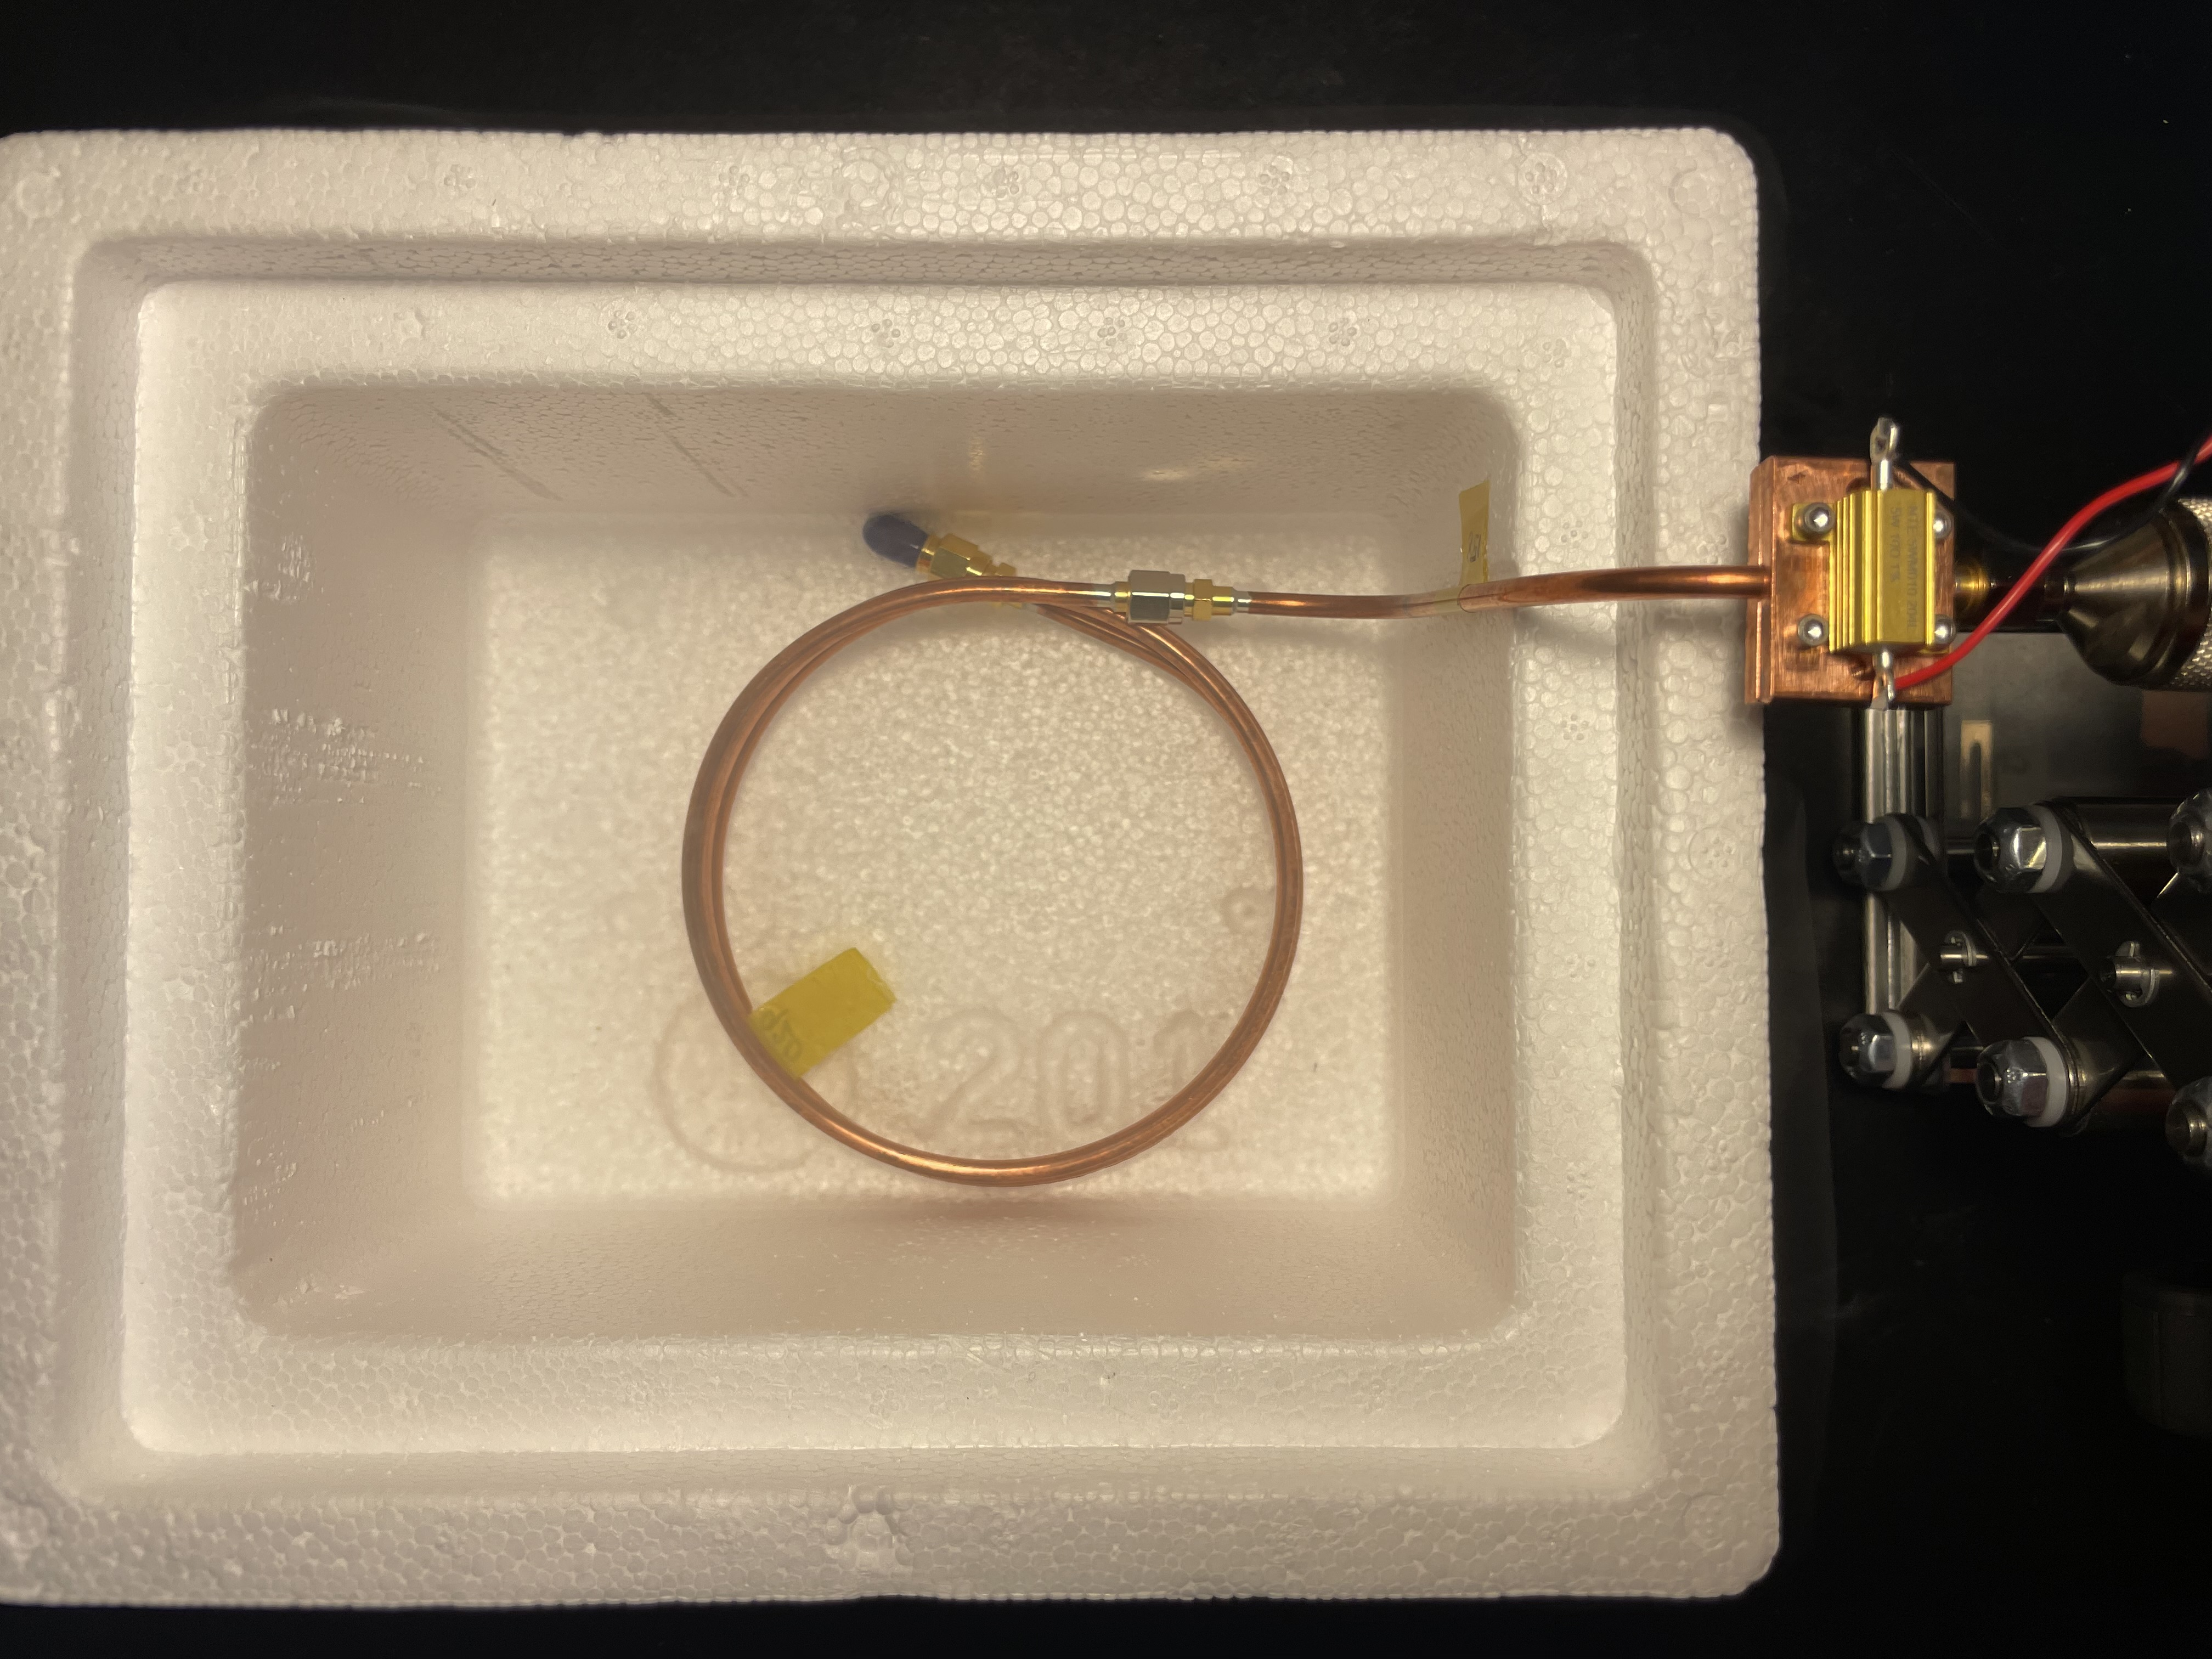
\includegraphics[width=0.75\linewidth]{figures/cold_Load.jpg}
	\caption{\LN{} cold termination measurement setup}
	\label{fig:cold_load}
\end{figure}

\section{Experimental Results} \label{sec:measurement}
\subsection{Noise Measurement Procedure}

Since the amplifier in this work is incredibly low noise, we measured the noise using the Y-factor method with a termination in liquid nitrogen (\LN{}) and a separate room-temperature termination.
If we know the atmospheric pressure, then we precisely know the boiling point of \LN{}.
Then, given the temperature of the cold termination, we need to consider the length of coax that exits the \LN{} bath, its frequency-dependent insertion loss, and its temperature gradient.
As the thermal conductivity of most materials is dependent on their temperature, the temperature gradient along the length of the coax line is nonlinear and must be solved numerically, as described in~\cite{solimanThermalModellingCoaxial2016}.

Next, we must consider the thermal load on the cold termination.
Even when submerged, heat from the warm side of the line will travel into the termination.
To reduce this effect, we could use a stainless steel line, as it has low thermal conductivity.
However, the temperature-dependent conductivity (and therefore insertion loss) of stainless steel is not well known.
Instead, we follow the submerged termination with a long length of line before exiting the bath.
In our case, we used an \qty{8}{\cm} section of RG402 coax connected to a submerged \qty{1}{\m} coil and termination.
We used a heater, shown in \autoref{fig:cold_load}, to maintain the warm end of the coax at ambient temperature.
Finally, we attached a previously characterized N to SMA adapter to the warm end of the cold load to mate with the N-type socket on the constructed LNA.
This setup, shown in \autoref{fig:cold_load}, has a frequency-dependent output noise following this curve-fit result:
%
\begin{equation}
	T_{\text{Cold}}\,\text{(K)} = 78.0824 + 1.2425f_{\si{\GHz}} -  0.1166f_{\si{\GHz}}^{2}
	\label{eqn:tcold}
\end{equation}
%
The error on this result depends on uncertainty in the length of the coax between the surface of the \LN{} and the heater (nominally \qty{8}{\cm}), the warm-side temperature (nominally \qty{297}{\K}), and the atmospheric pressure (nominally \qty{100}{\kilo\Pa}).
Assuming worst-case errors of \qty{\pm 1}{\cm} of length, \qty{\pm 2}{\C} in temperature, and \qty{\pm 0.5}{\kilo\Pa} of pressure, we derive an error model in frequency:
%
\begin{equation}
	\delta T_{\text{Cold}}\,\text{(K)} = 0.0776 + 0.0568f_{\si{\GHz}} - 0.0048f_{\si{\GHz}}^{2}
	\label{eqn:terr}
\end{equation}

\begin{figure}[t]
	\centering
	\begin{circuitikz}[european]
		\ctikzset{nodes width/.initial=0.1}
		\ctikzset{bipoles/length=0.8cm}
		\ctikzset{nodes width/.initial=.05}

		\draw
		(0,0) node[plain mono amp, font=\footnotesize] (dut) {DUT}
		(1.3,0) node[plain mono amp, font=\footnotesize] (rx_amp) {PA}
		(2.1,0) node[msport,circuitikz/RF/scale=2, font=\footnotesize](ADC) {RX}
		(dut.in) to[short] ++(-1.7,0) to[R,l_={$T_{H,C}$}] ++(0,-1) node[tlground]{}
		(dut.out) -- (rx_amp.in)
		(rx_amp.out) -- (ADC) ;

		%\draw[->]  (dut.in) ++(0,0.75) -- (2.1,0.75) node[midway,yshift=1em] {$G$};

		\draw [->, >=Stealth] (-1,-0.5) node[below]{$\Gamma_{\text{A}}$} |- (-0.7,-.1) ;
		\draw [->, >=Stealth] (-1.7,-0.5) node[below]{$\Gamma_{\text{S}_{H,C}}$} |- (-2.0,-.1);
		\draw [->, >=Stealth] (-1,0.5) node[above]{$T_A$} |- (-0.7,.1);

	\end{circuitikz}
	\caption[System schematic of the Y-factor measurement]{System schematic of the Y-factor measurement. The device under test (DUT) is presented a termination with reflection coefficients $\Gamma_{\text{S}_H}$ and $\Gamma_{\text{S}_C}$ at two temperatures $T_H$ and $T_C$, respectively. The DUT is followed by a series of preamplifiers (PA) before being digitized by the receiver (RX). The total noise temperature referred to the input of the DUT is $T_A$. The reflection coefficient at the input of the device under test is $\Gamma_\text{A}$}
	\label{fig:yfac_schematic}
\end{figure}

Finally, we must consider the errors due to changing source impedance between the hot and cold states.
These errors are present in all Y-factor measurements but are exacerbated in our \LN{} approach as there are two distinct terminations.
The impact on the measured Y-factor stems from two effects: the shift in the amplifier's effective input noise due to its noise parameters \eqref{eq:noise} and changes in available gain.

First, to use the Y-factor method, we must assume that the amplifier's noise remains constant between the two states, implying that the impact of the noise parameters is negligible.
Given that we measured both terminations to have return loss \qty{>=25}{\dB} and simulated $R_n$ \qty{<=2}{\ohm} and $|\Gamma_{\text{Opt}}|$ \num{<=0.6}, we expect no worse than \qty{0.03}{\K} error due to this assumption.

Next, we evaluate the impact due to changes in available gain.
Given a termination at the input of a noisy receiver, shown in \autoref{fig:yfac_schematic}, the output noise is given by
%
\begin{equation}
	P = k_{b}BD_\text{RX}G_\text{A}\left(T_{H,C}+T_\text{A}\right)
	\label{eq:noise_power}
\end{equation}
%
where $k_b$ is Boltzmann's constant, $B$ is the noise equivalent bandwidth, $D_\text{RX}$ is a scaling term capturing other digital and analog gain factors in the receiver, $T_{H,C}$ is the hot or cold noise temperature at the amplifier input, $T_\text{A}=T_\text{A}(\Gamma_{\text{S}_{H,C}})$ is the equivalent input noise temperature, and $G_\text{A} = G_\text{A}(\Gamma_{\text{S}_{H,C}})$ is the available gain of the amplifier given by
%
\begin{equation}
	G_{\text{A}} = \frac
	{|S_{21}|^{2}\left(1 - |\Gamma_{S}|^{2}\right)}
	{|1-\Gamma_{S}\Gamma_A|^{2} \left(1-|S_{22}|^2\right)}
\end{equation}
%
We write our expression for the measured Y-factor as a ratio of these hot and cold powers \cite{hpnoise1983}, but now without the assumption that $G_\text{A}$ remains constant due to the impact of $\Gamma_{\text{S}_{H,C}}$:
%
\begin{equation}
	Y =
	\frac
	{P_\text{H}}
	{P_\text{C}} =
	\frac
	{G_{\text{A,H}}\left(T_\text{H} + T_\text{A}\right)}
	{G_{\text{A,C}}\left(T_\text{C} + T_\text{A}\right)} =
	C\left(
	\frac
	{T_\text{H} + T_\text{A}}
	{T_\text{C} + T_\text{A}}
	\right)
	\label{eq:y_fac}
\end{equation}
%
where the correction $C$ due to mismatch error~\cite{heymannGuideNoiseMicrowave2021} is
%
\begin{equation}
	C =
	%\left(
	\frac
	{1 - |\Gamma_{S_\text{H}}|^{2}}
	{1 - |\Gamma_{S_\text{C}}|^{2}}
	%\right)
	%\left(
	\frac
	{|1-\Gamma_{S_\text{C}}\Gamma_A|^{2}}
	{|1-\Gamma_{S_\text{H}}\Gamma_A|^{2}}
	%\right)
\end{equation}
%
Solving \eqref{eq:y_fac} for $T_\text{A}$ yields:
%
\begin{equation}
	T_\text{A} = \frac{T_{\text{H}}-T_{\text{C}}Y/C}{Y/C-1}
	\label{eqn:corrected_yfac}
\end{equation}
%
This equation for noise temperature is identical to the standard expression, but with a correction term applied to Y.
Usually, this factor is close to unity, but as our amplifier is primarily designed for noise and not return loss, and the noise is exceptionally low, the interaction between $\GA$ and $\Gamma_\text{S}$ results in a nontrivial correction.
For our amplifier and terminations, $C$ is between \num{0.974} and \num{1.019}, representing a change in the computed noise of about \qtyrange{2}{4}{\K}, or a third of the total expected noise.

\begin{figure}[t]
	\centering
	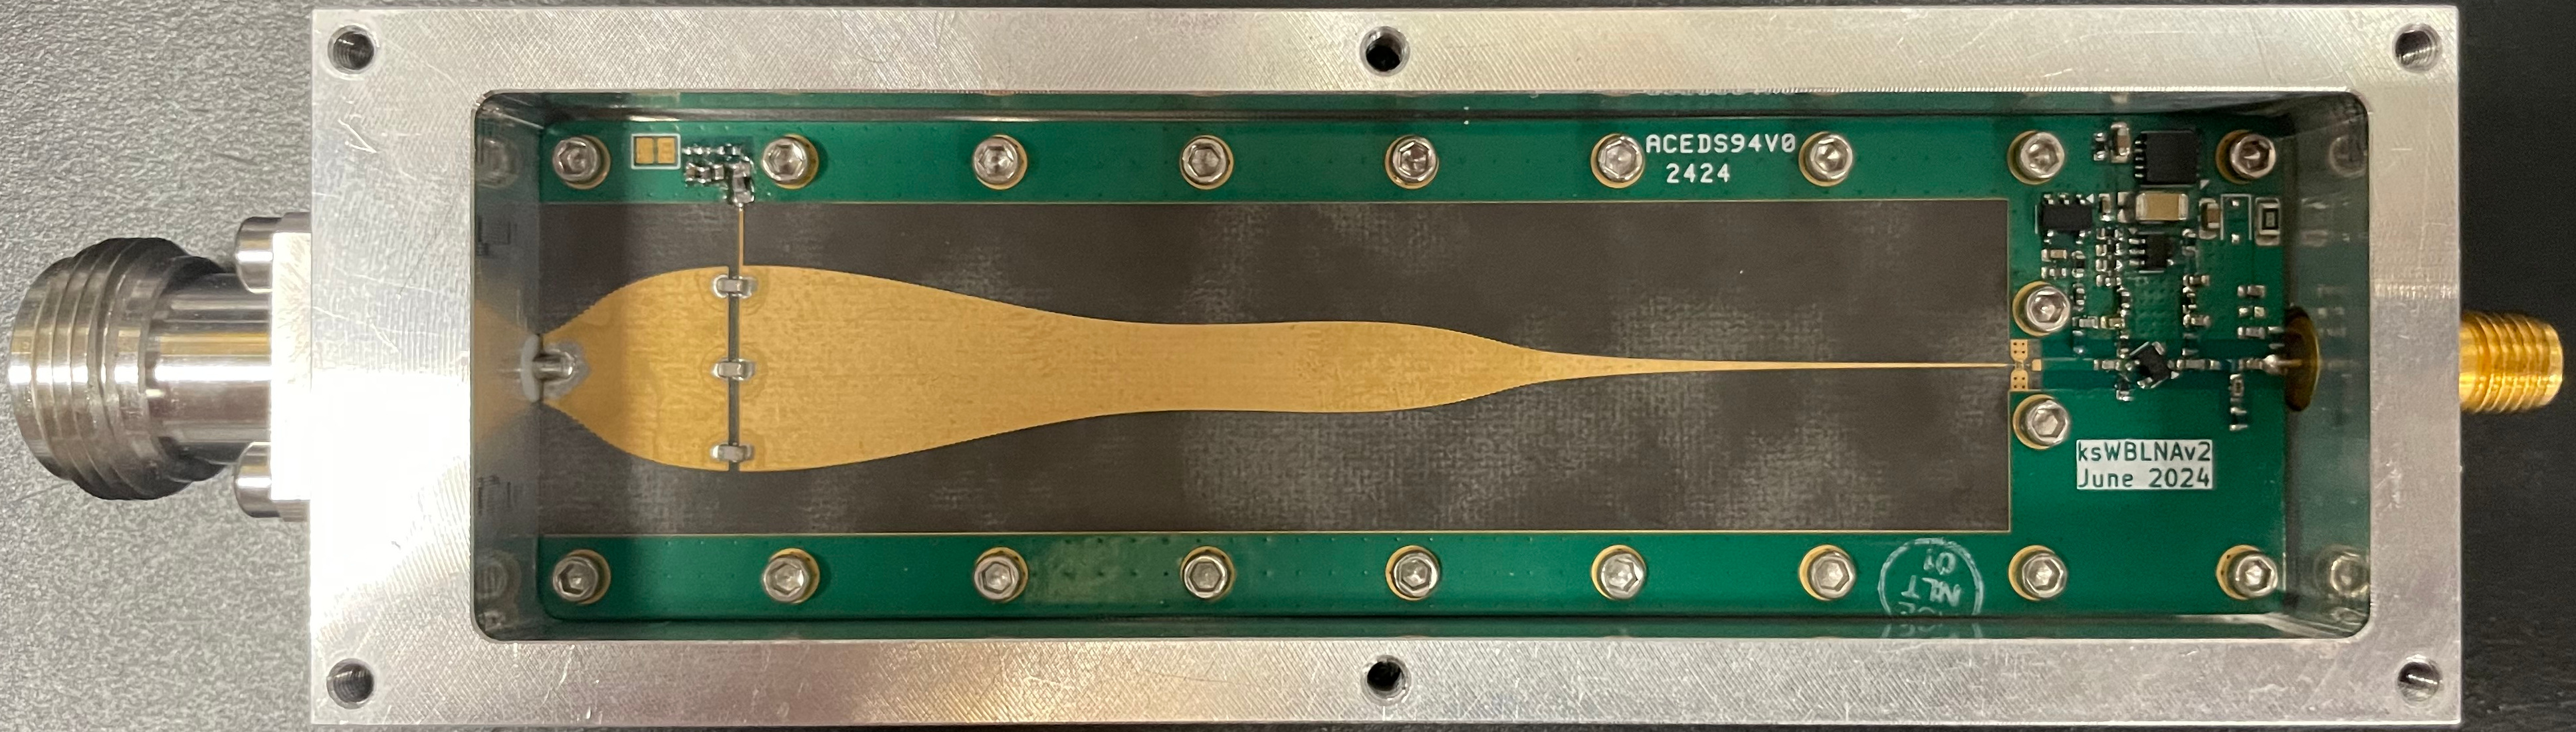
\includegraphics[width=\linewidth]{figures/LNA.jpg}
	\caption{The assembled amplifier in a machined aluminum enclosure with terminations and the lid removed}
	\label{fig:LNA}
\end{figure}

Additionally, we have uncertainty in the reflection coefficient measurements, which results in uncertainty in this correction factor.
Following the datasheet for our network analyzer~\cite{Keysight2Port4Port2018}, we create a curve-fit function to describe the uncertainty in both phase and magnitude, as a function of magnitude.
For our frequency range and IF bandwidth, these are:
\begin{equation}
	\delta|\Gamma| = 0.004 + 0.006|\Gamma|\left(1+|\Gamma|\right)
\end{equation}
and
\begin{equation}
	\delta\arg(\Gamma) = \frac{0.25^{\circ}}{|\Gamma|} + 0.5^{\circ}
\end{equation}

Finally, we need to remove the noise of the receiver.
We do so by performing a measurement with a room temperature termination on the receiver's input and subtracting the linear power from the hot and cold powers of the device under test.
We performed all these calculations also in the Julia language, making use of the \textit{Measurements.jl}~\cite{giordanoUncertaintyPropagationFunctionally2016} package to propagate uncertainty.

\clearpage
\begin{figure}[ht!]
	\centering
    
	\begin{tikzpicture}
		\begin{axis}[
				xlabel={Frequency (\si{\GHz})},
				ylabel={\si{\dB}},
				ymin=-40,ymax=0,
                xmin=0.7,xmax=2.1,
				width=13cm,
				height=6cm,
                xtick={},ytick={},
                minor tick num=1,
                grid=both,
                grid style={line width=.1pt, draw=gray!10},
                major grid style={line width=.2pt,draw=gray!50},
			]
			% S11
			\addplot[mark=none, very thick] table [x expr=\thisrow{freq}/1e9, y=s11, col sep=comma] {meas_s.csv};
			\addplot[mark=none, dashed, very thick] table [x expr=\thisrow{freq}/1e9, y=s11, col sep=comma] {sim_s.csv};
			% S22
			\addplot[mark=none, red, very thick] table [x expr=\thisrow{freq}/1e9, y=s22, col sep=comma] {meas_s.csv};
			\addplot[mark=none, red, dashed, very thick] table [x expr=\thisrow{freq}/1e9, y=s22, col sep=comma] {sim_s.csv};
            % Annotations
            \node[black, font=\footnotesize] at (axis cs: 1.15,-3) {$S_{11}$};
            \node[red, font=\footnotesize] at (axis cs: 1,-30) {$S_{22}$};
		\end{axis}
	\end{tikzpicture}
	\caption{Measured (solid) versus simulated (dashed) S parameters}
	\label{fig:s_compare_11_22}

    \begin{tikzpicture}
		\begin{axis}[
				xlabel={Frequency (\si{\GHz})},
				ylabel={\si{\dB}},
				ymin=34,ymax=40,
                xmin=0.7,xmax=2.1,
				width=13cm,
				height=6cm,
                xtick={},ytick={},
                minor tick num=1,
                grid=both,
                grid style={line width=.1pt, draw=gray!10},
                major grid style={line width=.2pt,draw=gray!50},
			]
            % S21
			\addplot[mark=none, black, very thick] table [x expr=\thisrow{freq}/1e9, y=s21, col sep=comma] {meas_s.csv};
			\addplot[mark=none, black, dashed, very thick] table [x expr=\thisrow{freq}/1e9, y=s21, col sep=comma] {sim_s.csv};
		\end{axis}
	\end{tikzpicture}
    \caption{Measured (solid) versus simulated (dashed) $S_{21}$}
    \label{fig:s_compare_21}

	\begin{tikzpicture}
		\begin{axis}[
				xlabel={Frequency (\si{\GHz})},
				ylabel={Noise Temperature (\si{\K})},
				ymin=8,ymax=17,
				xmin=0.7,xmax=2.1,
				width=13cm,
				height=6cm,
                xtick={},ytick={},
                minor tick num=1,
                grid=both,
                grid style={line width=.1pt, draw=gray!10},
                major grid style={line width=.2pt,draw=gray!50},
			]

			% KS LNA
			\addplot[mark=none, very thick] table [x=f, y=t, col sep=comma] {NTL.csv};
			\addplot [name path=upper,draw=none] table[x=f,y expr=\thisrow{t}+\thisrow{e}, col sep=comma] {NTL.csv};
			\addplot [name path=lower,draw=none] table[x=f,y expr=\thisrow{t}-\thisrow{e}, col sep=comma] {NTL.csv};
			\addplot [fill=black!10] fill between[of=upper and lower];

			% Simluated result
			\addplot[mark=none, dashed, very thick] table [x expr=\thisrow{freq} / 1e9, y=t, col sep=comma] {sim_data.csv};

			% SW LNA
			\addplot[mark=none, red, very thick] table [x=f, y=t, col sep=comma] {2-Step.csv};
			\addplot [name path=upper,draw=none] table[x=f,y expr=\thisrow{t}+\thisrow{e}, col sep=comma] {2-Step.csv};
			\addplot [name path=lower,draw=none] table[x=f,y expr=\thisrow{t}-\thisrow{e}, col sep=comma] {2-Step.csv};
			\addplot [fill=red!10] fill between[of=upper and lower];
		\end{axis}
	\end{tikzpicture}

	\caption{Measured (solid) and simulated (dashed) noise temperature of this work (lower trace), prior work~\cite{shiRoomTemperatureLowNoiseAmplifier2023} (higher trace), and 95\% confidence regions}
	\label{fig:noise_compare}
\end{figure}
\newpage
\subsection{Measured Results}

We measured the S parameters of the assembled amplifier (shown in \autoref{fig:LNA}) and the hot and cold terminations with a Keysight N5242A network analyzer with no averaging or smoothing.
We used a Siglent SSA3032X as the noise receiver, preceded by a Mini-Circuits ZX60-P105LN+ amplifier and bias tee.
We configured the spectrum analyzer to measure from \qtyrange{0.6}{2.1}{\GHz} with a resolution bandwidth of \qty{1}{\MHz}, video bandwidth of \qty{1}{\kHz}, attenuation of \qty{0}{\dB}, preamplifier enabled, and log power averaging.
After a \qty{30}{\minute} warm-up time, data were saved for the noise of the receiver and the device under test with the hot and cold terminations, recording the physical temperatures.
All measurements were performed at an ambient temperature of \qty{297}{\K}.
We performed these power measurements five times each, saving the batch mean and standard deviation.
In error analysis, we used these standard deviation data divided by $\sqrt{5}$ as the standard error of measurement.

We processed the measurements by computing the corrected Y-factor from \eqref{eqn:corrected_yfac}, including uncertainty.
Finally, these data were smoothed with a \qty{150}{\MHz} sliding window.
The results are shown in \autoref{fig:noise_compare}.
The average noise temperature from \qtyrange{0.7}{2}{\GHz} is \newnoise{}.
The measured S parameters match the simulation well, as shown in \autoref{fig:s_compare_11_22} and \autoref{fig:s_compare_21}, with disagreement in $S_{22}$ due to an un-modeled output connector interface.
$S_{21}$ is reasonably flat with \qty{>=35}{\dB} across the band and has a maximum of \qty{39}{\dB}, and $S_{11}$ is \qty{<=-8}{\dB}.
Differences between the simulated and measured $S_{11}$ and $S_{21}$ are due to imperfect wire bond geometry.

We performed these measurements on the amplifier from the prior work~\cite{shiRoomTemperatureLowNoiseAmplifier2023} using the same test setup, procedure, and physical temperature to ensure a fair comparison.
The results of this new measurement are also shown in \autoref{fig:noise_compare}.
Our measurements of the average noise temperature for the prior amplifier is \oldnoise.
Comparing the two amplifiers across the same frequencies, the presented design shows a \improvement mean improvement.
As shown in \autoref{tbl:amp_compare}, the presented amplifier outperforms not only the prior work in noise, but also other similar uncooled amplifiers intended for radio astronomy over a wide bandwidth.

\section{Conclusion}
In this chapter, we demonstrated the design of a non-uniform transmission line LNA input matching network using AD-accelerated gradient-based optimization.
This amplifier achieves a frequency-averaged noise temperature of \newnoise from \qtyrange{0.7}{2}{\GHz} at \qty{297}{\K}.
The NTL design outperforms a previous uniform-line design by \improvement.
This design method is algorithmically more efficient than finite-difference optimization, and outperforms such solvers by more than \num{40}x for this problem.
AD is a general-purpose method for computing derivates and could be adopted for many other microwave problems such as parameter estimation and sensitivity analysis, as well as inverse design of structures besides NTLs.

\begin{table}[h!]
    \centering
    \begin{threeparttable}
    \caption{Comparison of Similar Radio Astronomy LNAs}
    \label{tbl:amp_compare}
        \begin{tabular}{c c c c c}
             Ref. & Freq. (GHz) & $S_{21}$ (dB) & $T_{50}$\tnote{1} (K) &  Topo. / Tech. \\
             \hline& \\[-2.0ex]
             \textbf{This Work} & 0.7-2 & 36 & \num{11.5 \pm 0.4} & NTL / InP \\
             \cite{shiRoomTemperatureLowNoiseAmplifier2023} & 0.7-2 & 40 & \num{12.5 \pm 0.4}\tnote{2} & UTL / InP \\
            \cite{lai0315GHzLNAWideband2023} & 0.3-1.5 & 32 & \num{18 \pm 6} & Discrete / InP \\
            \cite{belostotskiSub02DBNoise2007} & 0.7-1.4 & 17 & 20 & CMOS \\
        \end{tabular}
        \begin{tablenotes}
            \item [1] Band-averaged noise temperature with a \qty{50}{\ohm} source impedance
            \item [2] Our measurements of this amplifier
        \end{tablenotes}
    \end{threeparttable}
\end{table}